\documentclass[12pt, a4paper]{article}
\usepackage{amsmath}
\usepackage{amsfonts}
\usepackage{amsthm}
\usepackage{mathtools}
\newtheorem{theorem}{Theorem}
\usepackage{pgfplots}
\pgfplotsset{width=10cm,compat=1.9}

\title{Bayesian inference}
\author{Kristian Wichmann}

\begin{document}

\maketitle

This document is based primarily on chapter 19 from Wonnacott and Wonnacott's "Introductory Statistics" (fifth edition) and the Coursera course "Bayesian Statistics" offered by Duke University.

\section{Basic Bayesian statistics}

\subsection{The Bayesian view of probability}

\textit{Bayesian statistics}, as opposed to frequentist statistics, views probabilities merely as current opinion regarding the true state of the world. As new data is brought to light such opinion will be revised to reflect the new evidence. The way to update probabilities is prescribed by Bayes' theorem.\par
So Bayesian probabilities are subjective, in contrast to the objective probabilities of frequentist statistics.

\subsection{Prior and posterior probabilities}
Assume we have a given probability of an event $A$ happening. This probability $P(A)$ is known as the \textit{prior} in Bayesian terminology. Now, assume we know that event $B$ has occured - this constitutes evidence. We should now adjust our probability of event $A$ to the conditional probability $P(A|B)$, which is known as the \textit{posterior}. The two are related by Bayes' theorem:
\begin{equation}
\label{bayes}
P(A|B)=\frac{P(B|A)P(A)}{P(B)}
\end{equation}

\subsubsection{Example: Radio quality}
A given corporation produces radios. Of the last 200 truckloads of radios, 128 have been "bad" and 72 "good"; In the bad truckloads 44\% of the radios were defective. In the good truckloads only 15\%. Now, we're faced with determining whether a new truckload of radios is good or bad. Initially, since all we have is the information that 128 out of 200 truckloads have been bad, our prior probabilities would be:
\begin{equation}
P(B)=\frac{128}{200}=64\%,\quad P(G)=\frac{72}{200}=36\%
\end{equation}
Here, $B$ refers to the event "Bad truckload", and $G$ to the event "Good truckload". However, we now sample one of the radios from the truckload. This radio turns out to be defective. What are the updated, posterior probabilities of the truckload being good or bad? To answer this, we need Bayes' theorem:
\begin{equation}
\label{radio_post}
P(B|D)=\frac{P(D|B)P(B)}{P(D)}
\end{equation}
Here $D$ refers to the event "Defective radio". $P(D|B)$ is the probability of a radio in a bad truckload being defective. We know that this is 44\%. We know that $P(B)=64\%$. But what is $P(D)$? By the law of total probability, this is:
\begin{equation}
P(D)=P(D|B)P(B)+P(D|G)P(G)=44\%\cdot 64\% + 15\%\cdot 36\% = 33.56\%
\end{equation}
Now, we can insert into equation $(\ref{radio_post})$:
\begin{equation}
P(B|D)=\frac{44\%\cdot 64\%}{33.56\%}=83.9\%
\end{equation}
By symmetry, the posterior probability of a good truckload has shrunk to $P(G|D)=100\%-83.9\%=16.1\%$. The knowledge that the sample radio is defect makes us update our view of the world.

\subsubsection{Radio quality with odds}
One could also reformulate the example above using \textit{odds}. The odds of a bad truckload is:
\begin{equation}
\frac{P(B)}{P(G)}=\frac{64\%}{36\%}=1.78
\end{equation} 
These are the prior odds. After the reveal of the defect radio, odds are:
\begin{equation}
\frac{P(B|D)}{P(G|D)}=\frac{83.9\%}{16.1\%}=5.21
\end{equation}
These are the posterior odds. How are the two related? Let's use Bayes' theorem to find out:
\begin{equation}
\frac{P(B|D)}{P(G|D)}=\frac{P(D|B)P(B)/P(D)}{P(D|G)P(G)/P(D)}=\frac{P(D|B)P(B)}{P(D|G)P(G)}
\end{equation}
So the prior odds times the quantity $\frac{P(D|B)}{P(G|B)}$, which can be interpreted as a \textit{likelihood ratio}. The relation between these three quantities can be written:
\begin{equation}
\label{bayes_odds}
\textrm{posterior odds}=\textrm{likelihood ratio}\cdot\textrm{prior odds}
\end{equation}

\subsection{Calculating posterior probabilities}
In general, let $\theta$ be a parameter (or a vector of parameters) used to describe an event. In the example above, $\theta$ covered two option: Good or Bad truckload. In general, $\theta$ may represent many - even infinitely many - different outcomes. Let $X$ represent new evidence. By Bayes' theorem:
\begin{equation}
P(\theta|X)=\frac{P(X|\theta)P(\theta)}{P(X)}
\end{equation}
For a given set of evidence $X$ we wish to update on, $P(X)$ is a constant, so this may also be expressed:
\begin{equation}
\label{bayes_prob}
P(\theta|X)\propto P(X|\theta)P(\theta)
\end{equation}
Or reworded to resemble equation $(\ref{bayes_odds})$:
\begin{equation}
\label{bayes_prob2}
\textrm{posterior probability}\propto\textrm{likelihood}\cdot\textrm{prior probability}
\end{equation}

\subsubsection{Discrete example: Coin throws}
Consider a coin which may or may not be biased. We initially think it's 50\% likely to be fair, but still consider the possibility of the probability of getting heads $p$ as 20\%, 40\%, 60\%, and 80\% possible, and assign each possibility an equal share of the remaining 50\%. In other words, our prior is:
\begin{center}
\begin{tabular}{ c | c c c c c }
 $p_0$		& 0.2 & 0.4 & 0.5 & 0.6	& 0.8 \\
 \hline
 $P(p=p_0)$	& $\frac{1}{8}$ & $\frac{1}{8}$ & $\frac{1}{2}$	& $\frac{1}{8}$ & $\frac{1}{8}$\\      
\end{tabular}
\end{center}
Now, we toss the coin three times and get all heads. What is the posterior distribution in this case? As usual, we can use Bayes' theorem to answer this:
\begin{equation}
P(p=p_0|3\textrm{ heads})=\frac{P(3\textrm{ heads}|p=p_0)P(p=p_0)}{P(3\textrm{ heads})}
\end{equation}
Here, $p_0$ may take on any of our five considered values. The likelihood $P(3\textrm{ heads}|p=p_0)$ is a binomial distribution:
\begin{equation}
P(3\textrm{ heads}|p=p_0)=\binom{3}{3}p_0^0(1-p_0)^3=(1-p_0)^3
\end{equation}
The probability $P(3\textrm{ heads})$ can be calculated using the law of total probability:
\begin{align*}
P(&3\textrm{ heads})=\sum_{p_0}P(3\textrm{ heads}|p=p_0)P(p=p_0)=\sum_{p_0}(1-p_0)^3 P(p=p_0)=\\
&(1-0.2)^3\frac{1}{8}+(1-0.4)^3\frac{1}{8}+(1-0.5)^3\frac{1}{2}+(1-0.6)^3\frac{1}{8}+(1-0.8)^3\frac{1}{8}=\\
&0.1625
\end{align*}
Now, we can calculate a posterior probability for each $p_0$. For instance:
\begin{equation}
P(p=0.2|3\textrm{ heads})=\frac{(1-0.2)^3\cdot\frac{1}{8}}{0.1625}\approx 39.4\%
\end{equation}
Repeating for the remaining 4 possibilities gives us the following table of the posterior distribution:
\begin{center}
\begin{tabular}{ c | c c c c c }
 $p_0$		& 0.2 & 0.4 & 0.5 & 0.6	& 0.8 \\
 \hline
 $P(p=p_0|3\textrm{ heads})$ & 39.4\% & 16.6\% & 38.5\%	& 4.9\% & 0.6\%\\      
\end{tabular}
\end{center}
Of course, we could also have disregarded the constants independent of $p_0$ - the denominator and the binomial coefficient (in generel it will be different from 1) - and eventually normalize the resulting distribution.

\subsubsection{Discrete example: The "two-armed bandit"}
We have two slot machines - also known as "one-armed bandits" - to play. Let's call them $M_1$ and $M_2$. We know that one of them is "good", in that the win rate is $\frac{1}{2}$, and that one of them is "bad", having only a win rate of $\frac{1}{3}$. But initially, we do not know which is which. So our prior is:
\begin{equation}
P(M_1\textrm{ good}=P(M_2\textrm{ bad})=\frac{1}{2},\quad P(M_1\textrm{ bad})= (M_2\textrm{ good})=\frac{1}{2}
\end{equation}
But we do know the conditional probabilities for winning
\begin{align}
P(\textrm{Win on }M_1|M_1\textrm{ good})=&P(\textrm{Win on }M_2|M_2\textrm{ good})=\frac{1}{2}\\
P(\textrm{Win on }M_1|M_1\textrm{ bad})=&P(\textrm{Win on }M_2|M_2\textrm{ bad})=\frac{1}{3}
\end{align}
And losing:
\begin{align}
P(\textrm{Lose on }M_1|M_1\textrm{ good})=&P(\textrm{Lose on }M_2|M_2\textrm{ good})=\frac{1}{2}\\
P(\textrm{Lose on }M_1|M_1\textrm{ bad})=&P(\textrm{Lose on }M_2|M_2\textrm{ bad})=\frac{2}{3}
\end{align}
Now, let's say that we play $M_1$ and we win. What is the posterior probability of $M_1$ being good? We use Bayes' theorem:
\begin{align}
&P(M_1\textrm{ good}|\textrm{Win on }M_1)=\\
&\frac{P(\textrm{Win on }M_1|M_1\textrm{ good})P(M_1\textrm{ good})}{P(\textrm{Win on }M_1|M_1\textrm{ good})P(M_1\textrm{ good})+P(\textrm{Win on }M_1|M_1\textrm{ bad})P(M_1\textrm{ bad})}
\end{align}
This is equal to:
\begin{equation}
\frac{\frac{1}{2}\cdot\frac{1}{2}}{\frac{1}{2}\cdot\frac{1}{2}+\frac{1}{3}\cdot\frac{1}{2}}=\frac{1/4}{5/12}=\frac{3}{5}=60\%
\end{equation}
This also means, that the posterier probability of $M_2$ being good is 40\%. If we had instead played $M_1$ and lost the corresponding posterior would be:
\begin{align}
&P(M_1\textrm{ good}|\textrm{Lose on }M_1)=\\
&\frac{P(\textrm{Lose on }M_1|M_1\textrm{ good})P(M_1\textrm{ good})}{P(\textrm{Lose on }M_1|M_1\textrm{ good})P(M_1\textrm{ good})+P(\textrm{Lose on }M_1|M_1\textrm{ bad})P(M_1\textrm{ bad})}
\end{align}
This is equal to:
\begin{equation}
\frac{\frac{1}{2}\cdot\frac{1}{2}}{\frac{1}{2}\cdot\frac{1}{2}+\frac{2}{3}\cdot\frac{1}{2}}=\frac{1/4}{7/12}=\frac{3}{7}\approx 42.9\%
\end{equation}
Now, what about several plays, possibly on both machines? Let's say that you play $M_1$, $n_1$ times, winning $w_1$ times and losing $l_1$ times (so $n_1=w_1+_1$) and similarly $n_2, w_2$ and $l_2$ for $M_2$. In this case, the likelihood becomes a product of binomials. For instance, if we're looking for the posterior of $M_1$ being good, we will need the following likelihood:
\begin{equation}
P(w_1,l_1;w_2,l_2|M_1\textrm{ good})=\binom{n_1}{w_1}\left(\frac{1}{2}\right)^{w_1}\left(\frac{1}{2}\right)^{l_1}\cdot\binom{n_2}{w_2}\left(\frac{1}{3}\right)^{w_2}\left(\frac{2}{3}\right)^{l_1}
\end{equation}
The similar likelihood corresponding to $M_2$ being good would be:
\begin{equation}
P(w_1,l_1;w_2,l_2|M_2\textrm{ good})=\binom{n_1}{w_1}\left(\frac{1}{3}\right)^{w_1}\left(\frac{2}{3}\right)^{l_1}\cdot\binom{n_2}{w_2}\left(\frac{1}{2}\right)^{w_2}\left(\frac{1}{2}\right)^{l_1}
\end{equation}
As an example, let's consider the case where we play $M_1$ twice, winning both times, and play $M_2$ three times, winning twice and losing once. This corresponds to $n_1=2, w_1=2, l_1=0, n_2=3, w_1=2, l_2=1$. Plugging in:
\begin{align*}
P(&w_1=2,l_1=0;w_2=2,l_2=1|M_1\textrm{ good})=\\
&\binom{2}{2}\left(\frac{1}{2}\right)^2\left(\frac{1}{2}\right)^0\cdot\binom{3}{2}\left(\frac{1}{3}\right)^2\left(\frac{2}{3}\right)^1=1\cdot\frac{1}{4}\cdot 1\cdot 3\cdot\frac{1}{9}\cdot\frac{2}{3}=\frac{1}{18}\\
P(&w_1=2,l_1=0;w_2=2,l_2=1|M_2\textrm{ good})=\\
&\binom{2}{2}\left(\frac{1}{3}\right)^2\left(\frac{2}{3}\right)^0\cdot\binom{3}{2}\left(\frac{1}{2}\right)^2\left(\frac{1}{2}\right)^1=1\cdot\frac{1}{9}\cdot 1\cdot 3\cdot\frac{1}{4}\cdot\frac{1}{2}=\frac{1}{24}
\end{align*}
Starting from the same prior as above, we need the two expressions:
\begin{align*}
P(w_1=2,l_1=0;w_2=2,l_2=1|M_1\textrm{ good})P(M_1\textrm{ good})&=\frac{1}{18}\cdot\frac{1}{2}=\frac{1}{36}\\
P(w_1=2,l_1=0;w_2=2,l_2=1|M_2\textrm{ good})P(M_2\textrm{ good})&=\frac{1}{24}\cdot\frac{1}{2}=\frac{1}{48}
\end{align*}
To get the posteriors, these should be normalized. The sum is $\frac{1}{36}+\frac{1}{48}=\frac{7}{144}$. This means that the posterior probabilities are:
\begin{align*}
P(M_1\textrm{ good}|w_1=2,l_1=0;w_2=2,l_2=1)&=\frac{1/36}{7/144}=\frac{4}{7}\approx 57.1\%\\
P(M_2\textrm{ good}|w_1=2,l_1=0;w_2=2,l_2=1)&=\frac{1/48}{7/144}=\frac{3}{7}\approx 42.9\%
\end{align*}

\subsubsection{Continuous example: Radio quality revisited}
The radio manufacturing company from above have made further inquiries into the distribution of percentages of defective radios in a truckload. In this situation, the general parameter $\theta$ from last section corresponds to the defective percentage, which we will call $\pi$. It turns out, that this percentage seems to follow a beta distribution with parameters $\alpha=2$ and $\beta=4$:
\begin{equation}
P(\pi)\propto\pi(1-\pi)^3
\end{equation}
Since beta distributions are continuous, this is a probability \textit{density} of finding a truckload with a defective percentage of $\pi$, rather than a probability - this is our prior. We're now presented with a new truckload of radios. Without any further information, our best bet is the prior distribution. However, we now inspect the truckload, taking a random sample of 5 radios. It turns out, that 3 of those are defective. How do we account for this new information to update our distribution? According to equation $(\ref{bayes_prob})$, we need to find the likelihood $P(X|\pi)$. Here $X$ refers to the evidence of getting 3 out of 5 defective radios. In other words, this is a binomial likelihood\footnote{This assumes that the truckload is large enough that the consecutive picking of radios to test does not affect $\pi$ significantly.}:
\begin{equation}
P(X|\pi)=\binom{5}{3}\pi^3(1-\pi)^2\propto\pi^3(1-\pi)^2
\end{equation}
So the posterior distribution also turns out to be a beta distribution:
\begin{equation}
P(\pi|X)\propto\pi^4(1-\pi)^5
\end{equation}
This is a beta distribution with parameters $\alpha=5$ and $\beta=6$. The graph below shows the three distributions for comparison\footnote{The likelihood isn't a distribution, since it does not sum to 1. However, for clarity, in this figure it has been scaled as if it did.}. The prior is relatively optimistic regarding quality, and the likelihood less so. The posterior is a compromise between the two.

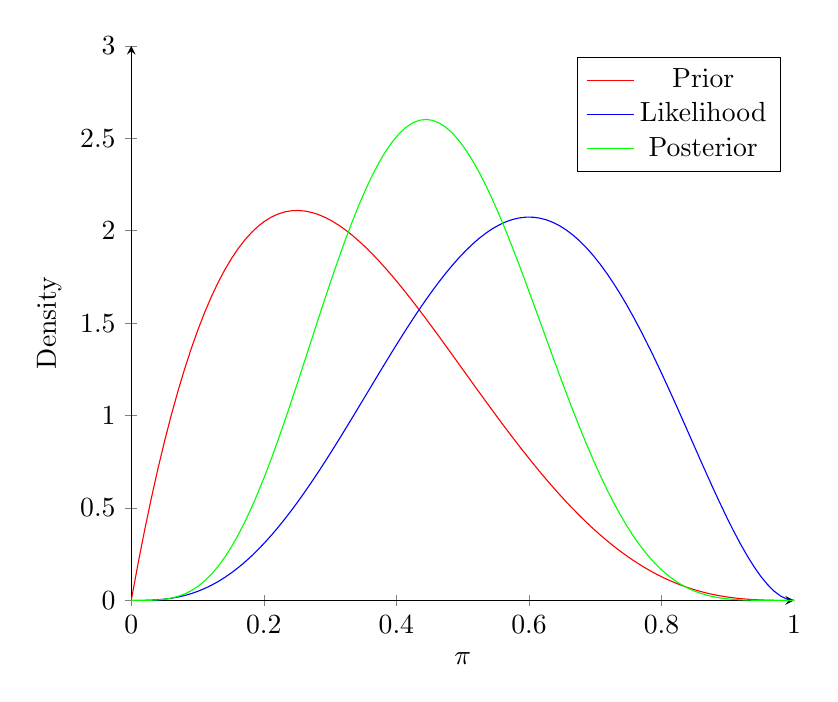
\begin{tikzpicture}
\begin{axis}[
    axis lines = left,
    xlabel = $\pi$,
    ylabel = Density,
    ymin = 0,
    ymax = 3,
]
\addplot [
    domain=0:1, 
    samples=100, 
    color=red,
]
{20 * x * (1-x)^3};
\addlegendentry{Prior}
\addplot [
    domain=0:1, 
    samples=100, 
    color=blue,
    ]
    {60 * x^3 * (1-x)^2};
\addlegendentry{Likelihood}
\addplot [
    domain=0:1, 
    samples=100, 
    color=green,
    ]
    {1260 * x^4 * (1-x)^5};
\addlegendentry{Posterior}
 
\end{axis}
\end{tikzpicture}

\subsection{Conjugate priors}
Usually, our assumption will be that the likelihood function of the data takes on a certain form. For instance, in the example above, the likelihood function was a binomial. In this case, we saw that a prior following a beta distribution also lead to a posterior following a beta distribution. Since both distributions are of the same type, we call them \textit{conjugate distributions}. Given a family of likelihood functions, a prior that makes the distributions conjugate is known as a \textit{conjugate prior} to the likelihood. So, for instance, the beta is a conjugate prior to the binomial.

\section{Beta as conjugate prior to binomial}
We've already seen the beta distribution in action in the example above. The distribution is useful, because it's appropriate to assign to something that is itself a probability, which is often the case with parameters in Bayesian statistics.

\subsection{Beta as prior and posterior}
Assume posterior distribution is a beta distribution with parameters $\alpha$ and $\beta$. If the evidence consists of $S$ successes and $F$ failures, then the math in the example easily generalizes, and we get that the posterior is again a beta distribution with parameters $\alpha+S$ and $\beta+F$. Which shows that the beta is a conjugate prior to the binomial.

\subsection{The prior as a quasi-sample}
Assume we have no previous information on the distribution, so that our prior a uniform. This corresponds to $\alpha=\beta=1$. If the evidence is $S$ successes and $F$ failures, the posterior is a beta distribution with parameters $S+1$ and $F+1$. This shows that the information contained in the prior is equivalent to having observed $\alpha-1$ successes and $\beta-1$ failures. So information-wise, the prior can be regarded as a \textit{quasi-sample} with $\alpha+\beta-2$ \textit{quasi-observations} in it.

\subsubsection{Example: Radio quality revisited}
In the example above, the prior has parameters $\alpha=2$ and $\beta=4$. This means that the prior is equivalent to $2+4-2=4$ observations, one being a defective radio, and three being functional.

\section{Gamma as conjugate prior to Poisson}
Sometimes, however, the parameter associated with the likelihood is not a probability. A prime example is the Poisson distribution. Remember that the Poisson distribution shows the probability of a number of independent "extraordinary events" in a given time interval. The probability mass function is:
\begin{equation}
P(j)=\frac{\lambda^j}{j!}e^{-\lambda},\quad n\in\mathbb{N}_0
\end{equation}
Here, the parameter $\lambda$ is the average number of events in the time interval\footnote{It also happens to be the variance of the distribution.}. $\lambda$ can take on any positive value, so we're looking for a family of distributions that reflects this.

\subsection{Gamma as prior and posterior}
It turns out that the family of gamma distributions is a good choice here. Recall, that a gamma distribution has two parameters $\alpha$ and $\beta$. However, here we will use the parametrization $k=\alpha$ and $\theta=\frac{1}{\beta}$. With these parameters, the probability density function is:
\begin{equation}
\label{gamma}
f(\lambda)=\frac{1}{\theta^k \Gamma(k)}\lambda^{k-1}e^{-\lambda/\theta}
\end{equation}
The mean turns out to be $k\theta$ and the variance $\theta\sqrt{k}$. Now, assume a prior of the form above and let $j_1, j_2,\cdots,j_n$ represent new evidence. Then Bayes' theorem tells us that the posterior is:
\begin{align}
P(k,\theta|j_1, j_2,\cdots,j_n)&\propto P(j_1, j_2,\cdots,j_n|k,\theta)P(k,\theta)\propto\\
\prod_{i=1}^n\left(\lambda^{j_i}e^{-\lambda}\right)\lambda^{k-1}e^{-\lambda/\theta}&=\lambda^{k+\sum_{i=1}^n j_i-1}e^{-n\lambda-\lambda/\theta}
\end{align}
This is a integration kernel of the same form as in equation $(\ref{gamma})$, so this must also be a gamma distribution. We can rewrite:
\begin{equation}
n\lambda+\frac{\lambda}{\theta}=\lambda\left(n+\frac{1}{\theta}\right)=\lambda\frac{n\theta+1}{\theta}
\end{equation}
So the posterior parameters are:
\begin{equation}
\label{gamma_poisson_posterior}
k^*=k+\sum_{i=1}^n j_i,\quad\theta^*=\frac{\theta}{n\theta+1}
\end{equation}

\subsubsection{Posterior in terms of $\alpha$ and $\beta$}
When expressing the gamma distribution in terms of the parameters $\alpha$ and $\beta$, the updating formula is a bit different (and actually simpler). Since $k=\alpha$, this remains the same. But for $\beta=1/\theta$ we have:
\begin{equation}
\beta^*=\frac{1}{\theta^*}=\frac{n(1/\beta)+1}{1/\beta}=n+\beta
\end{equation}
To sum it up:
\begin{equation}
\alpha^*=\alpha+\sum_{i=1}^n j_i,\quad\beta^*=\beta+n
\end{equation}

\subsection{Example: Workplace accidents}
A company keeps a record of major workplace accidents. After 5 years, they've found that a gamma distribution with parameters $k=7$ and $\theta=1/5$ is a reasonable prior for the parameter $\lambda$. Three years later, they've recorded two major accidents during this timespan. This corresponds to a likelihood function of:
\begin{equation}
P(\lambda|2\textrm{ accidents in }3\textrm{ years})\propto \lambda^{2}e^{-3\lambda}
\end{equation}
The corresponding mean is $k\theta=7/5=1.4$ and the variance $\theta\sqrt{k}\approx 0.53$. According to equation $(\ref{gamma_poisson_posterior})$ the posterior distribution has the parameters:
\begin{equation}
k^*=7+2=9,\quad\theta^*=\frac{1/5}{3\cdot 1/5+1}=\frac{1/5}{8/5}=\frac{1}{8}
\end{equation}
The posterior mean is $\frac{9}{8}=1.125$ and the variance $\frac{3}{8}=0.375$. The graph below shows the three distributions.

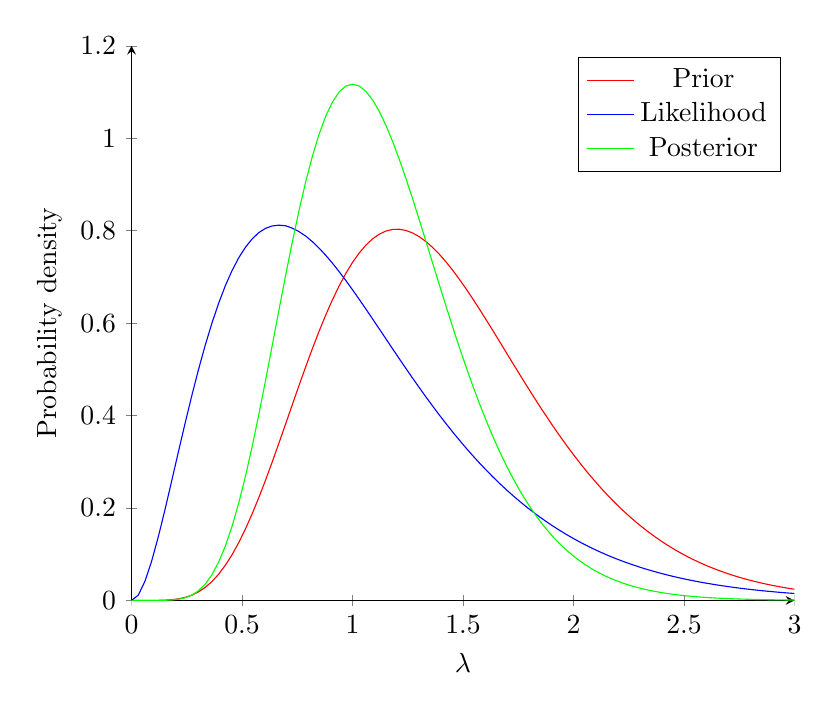
\begin{tikzpicture}
\begin{axis}[
    axis lines = left,
    xlabel = $\lambda$,
    ylabel = Probability density,
    ymin = 0,
    ymax = 1.2,
]
\addplot [
    domain=0:3, 
    samples=100, 
    color=red,
	]
	{x^6 * pow(2.71828,-5*x) * 78125 / 720};
\addlegendentry{Prior}
\addplot [
    domain=0:3, 
    samples=100, 
    color=blue,
    ]
    {x^2 * pow(2.71828,-3*x) * 27 / 2};
\addlegendentry{Likelihood}
\addplot [
    domain=0:3, 
    samples=100, 
    color=green,
    ]
    {x^8 * pow(2.71828,-x * 8) * 134217728 / 40320};
\addlegendentry{Posterior}
 
\end{axis}
\end{tikzpicture}


\subsection{Example: Cavalrists kicked to death by horses}
The Russian statician Ladislaus Bortkiewicz famously analyzed data from fifteen Prussian cavalry units. He showed that the yearly numbers of cavalrists kicked to death by their own horses followed a Poisson distribution. Which makes sense, since it counts the number of extraordinary events during the fixed time period of year. Let's assume a general, who assesses that the average number of soldiers kicked to death in a unit pr. year is 0.75, and that the variance of this number is 1. The corresponding $k$ and $\theta$ are found by solving:
\begin{equation}
k\theta=\frac{3}{4},\quad\theta\sqrt{k}=1
\end{equation}
The solution is $k=\frac{9}{16}$ and $\theta=\frac{4}{3}$. Now, after recording data for a total of 300 cavalry unit-years, he find a total of 200 soldiers kicked to death by their own horses. This means that the likelihood is:
\begin{equation}
P(\lambda|\textrm{evidence})\propto\lambda^{200}e^{-300\lambda},\quad n\in\mathbb{N}_0
\end{equation}
According to equation $\ref{gamma_poisson_posterior}$ his posterior parameters are then:
\begin{equation}
k^*=\frac{9}{16}+200=\frac{3209}{16}\approx 200.56,\quad\theta^*=\frac{\frac{4}{3}}{300\cdot\frac{4}{3}+1}=\frac{4}{1203}\approx 0.0033
\end{equation}
The corresponding mean and variance is:
\begin{equation}
\textrm{Mean: }k^*\theta^*\approx0.67,\quad\textrm{Variance: }\theta^*\sqrt{k^*}\approx 0.047
\end{equation}
So, the general's new estimate is somewhat lower, but much more precise, with a new standard deviation of $\sqrt{0.047}=0.22$, about a fourth of the prior. The graph below shows the three distributions.

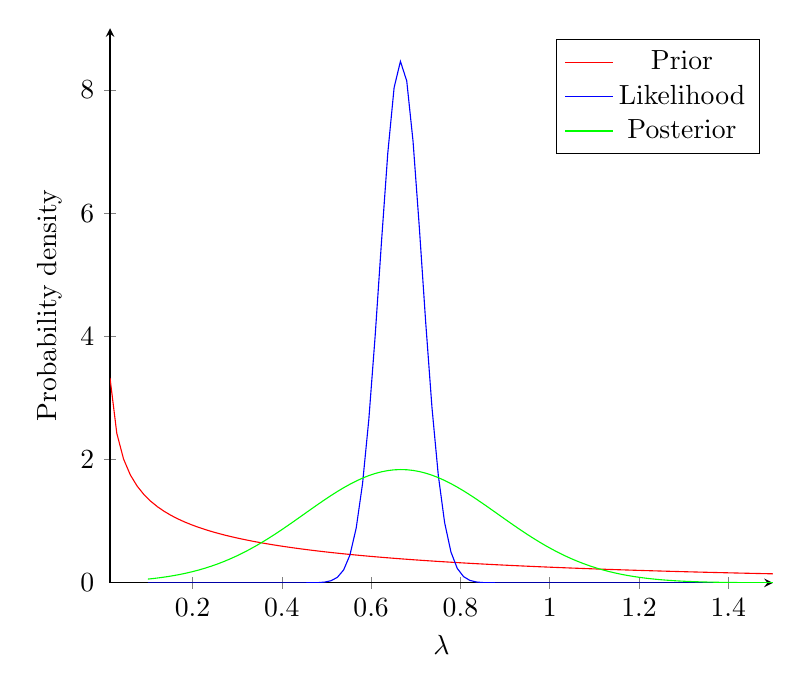
\begin{tikzpicture}
\begin{axis}[
	domain=0:1.5, restrict y to domain=-10:10,    
    axis lines = left,
    xlabel = $\lambda$,
    ylabel = Probability density,
    ymin = 0,
    ymax = 9,
]
\addplot [
    samples=100, 
    color=red,
	]
	{0.5377 * e^(-3*x/4) / x^(7/16)};
\addlegendentry{Prior}
\addplot [
    domain=0.1:1.5, 
    samples=100, 
    color=blue,
    ]
    {8.463 * e^(-(x - 2/3)^2 / (2 * 0.002222))};
\addlegendentry{Likelihood}
\addplot [
    domain=0.1:1.5, 
    samples=100, 
    color=green,
    ]
    {1.838 * e^(-(x - 0.66687)^2 / (2 * 0.047089))};
\addlegendentry{Posterior}
 
\end{axis}
\end{tikzpicture}

\subsection{The prior as quasi-sample}
Like we did in the beta-binomial case, we may also think of the prior as containing information comparable to the sample. Here, a prior with parameters $k$ and $\theta$ corresponds to $k$ quasi-observations over $1/\theta$ periods. When considering the update rules in the $\alpha, \beta$-parametrization, this is especially clear.

\subsubsection{Example: Workplace accidents}
Here, the prior is equivalent to 7 accidents over the 5 years. Compared to the samples 2 accidents over 3 years, both are important for the posterior, though the prior weighs a little heavier.

\subsubsection{Example: Cavalrists kicked to death by horses}
The prior now corresponds to $9/16$ observations over $4/3$ cavalry-years. Compared to the 200 observations over 300 cavalry-years in the sample, it is clear why the posterior is so close to the likelihood.

\section{Normal as conjugate prior to normal with known $\sigma^2$}
Let's assumme we're in a situation where we have good reason to suspect that a parameter is normally distributed with a known variance $\sigma^2$, but where the mean $\mu$ is unknown. So, when considering a prior for the parameter $\mu$ we need a distribution that can take on any real values. It turns out, that using a normal distribution for the prior will yield a normal posterior as well.

\subsection{Normal as prior and posterior}
Assume our prior is a normal distribution with mean $\nu$ and variance $\tau^2$. The associated probability density function is:
\begin{equation}
f(\mu)=\frac{1}{\sqrt{2\pi\tau^2}}\exp\left(-\frac{(\mu-\nu)^2}{2\tau^2}\right)
\end{equation}
Now, we're presented with evidence in the form of $x_1,x_2,\cdots,x_n$. The posterior distribution is given by Bayes' theorem:
\begin{equation}
P(\mu|x_1,x_1,x_2,\cdots,x_n)\propto P(x_1,x_2,\cdots,x_n|\mu)P(\mu)
\end{equation}
The likelihood is determined by the mean of the observations $\bar{x}=\frac{1}{n}\sum_{i=1}^n x_i$, since this is known to be normally distributed with mean $\mu$ and variance $\frac{\sigma^2}{n}$:
\begin{equation}
P(x_1,x_2,\cdots,x_n|\mu)=P(\bar{x}|\mu)\propto\exp\left(-\frac{(\mu-\bar{x})^2}{2\sigma^2/n}\right)
\end{equation}
Now, we can calculate the posterior:
\begin{equation}
P(\mu|\bar{x})\propto\exp\left(-\frac{(\mu-\bar{x})^2}{2\sigma^2/n}\right)\exp\left(-\frac{(\mu-\nu)^2}{2\tau^2}\right)
\end{equation}
We now use the general result, that the product of two normal pdf's with parameters $(\mu_1,\sigma_1^2)$ and $(\mu_2,\sigma_2^2)$ respectively, is proportional to a normal pdf with mean and standard deviation:
\begin{equation}
\mu^*=\frac{\sigma_1^2\mu_2+\sigma_2^2\mu_1}{\sigma_1^2+\sigma_2^2},\quad\sigma^*=\frac{\sigma_1\sigma_2}{\sqrt{\sigma_1^2+\sigma_2^2}}
\end{equation}
Inserting $\mu_1=\bar{x}, \sigma_1=\sigma/\sqrt{n}, \mu_2=\nu$ and $\sigma_2=\tau$ we get:
\begin{equation}
\mu^*=\frac{\frac{\sigma^2}{n}\nu+\tau^2\bar{x}}{\frac{\sigma^2}{n}+\tau^2},\quad\sigma^*=\frac{\frac{\sigma}{\sqrt{n}}\tau}{\sqrt{\frac{\sigma^2}{n}+\tau^2}}
\end{equation}
Simplify $\mu^*$:
\begin{equation}
\label{posterior_mu_formula}
\mu^*=\frac{\nu\sigma^2+n\tau^2\bar{x}}{n}/\frac{\sigma^2+n\tau^2}{n}=\frac{\nu\sigma^2+n\tau^2\bar{x}}{\sigma^2+n\tau^2}
\end{equation}
And $\sigma^*$:
\begin{equation}
\label{posterior_sigma_formula}
\sigma^*=\frac{\sigma\tau}{\sqrt{\sigma^2+n\tau^2}}=\sqrt{\frac{\sigma^2\tau^2}{\sigma^2+n\tau^2}}
\end{equation}
All in all, this means that the posterior can be written:
\begin{equation}
P(\mu|\bar{x})\propto\exp\left(-\frac{(\mu-\mu^*)^2}{2(\sigma^*)^2}\right)
\end{equation}

\subsection{Example: Steel beam strength}
Steelco makes thousands of shipments of steel beams. The breaking strength of a shipments is normally distributed within the shipment, with a standard deviation of $\sigma=17.3$, but due to poor quality control, the means $\mu$ varies from shipment to shipment. However, the mean is well known to be normally distributed around a mean of $\nu=60$ with a standard deviation of $\tau=10$. This is our prior. We now inspect a specific shipment of steel beams. After sampling 12 beams randomly, we find the sample mean to be $\bar{x}=70$. So the likelihood has mean 70 and standard deviation $17.3/\sqrt{12}\approx 4.99$. What is the posterior distribution? We can calculate the parameters using equations $(\ref{posterior_mu_formula})$ and $(\ref{posterior_sigma_formula})$:
\begin{align}
\mu^*=\frac{60\cdot 17.3^2+12\cdot 10^2\cdot 70}{17.3^2+12\cdot 10^2}&\approx 68.00\\
\sigma^*=\sqrt{\frac{17.3^2\cdot 10^2}{17.3^2+12\cdot 10^2}}&\approx 4.47
\end{align}

The pictures below graphs the three distributions\footnote{Again, the likelihood is not a distribution, but it has been normalized for easy comparison to the prior and posterior.}.

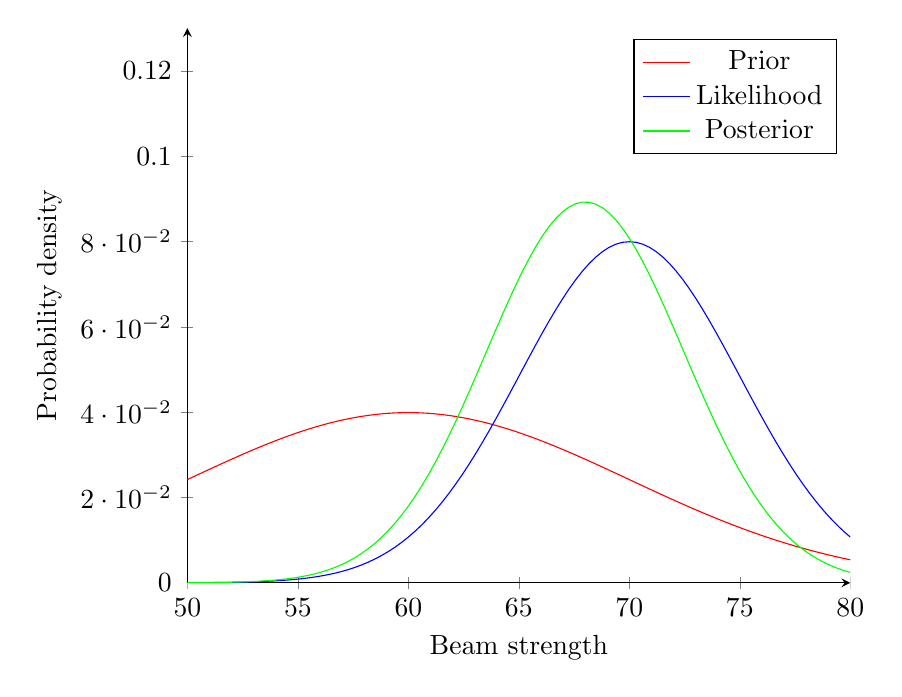
\begin{tikzpicture}
\begin{axis}[
    axis lines = left,
    xlabel = Beam strength,
    ylabel = Probability density,
    ymin = 0,
    ymax = 0.13,
]
\addplot [
    domain=50:80, 
    samples=100, 
    color=red,
	]
	{(pow(2.71828, -(x - 60)^2 / (2 * 10^2)) / (pow(2 * 3.14159, 0.5) * 10)};
\addlegendentry{Prior}
\addplot [
    domain=50:80, 
    samples=100, 
    color=blue,
    ]
    {(pow(2.71828, -(x - 70)^2 / (2 * 4.99^2)) / (pow(2 * 3.14159, 0.5) * 4.99)};
\addlegendentry{Likelihood}
\addplot [
    domain=50:80, 
    samples=100, 
    color=green,
    ]
    {(pow(2.71828, -(x - 68)^2 / (2 * 4.47^2)) / (pow(2 * 3.14159, 0.5) * 4.47)};
\addlegendentry{Posterior}
 
\end{axis}
\end{tikzpicture}

Again, we see that the posterior is a compromise between the prior and the likelihood. Also, the evidence has lowered the standard deviation. The following section shows a more extreme example of this.

\subsection{Example: Weighing ammonium nitrate}
An analytical chemist is going to weigh a sample of ammonium nitrate. She knows that the scale she is using has a standard deviation of 0.2 mg. Looking at the sample, she estimates it to weigh about 10 mg, while assigning a standard deviation on that guess to 2 mg. In other words, her prior is the normal distribution $N(10, 2)$. Now, she weighs the sample 5 times, getting an average weight of 10.5 mg. So the likelihood standard deviation is $0.2/\sqrt{5}\approx 0.089$. Her posterior distribution for the sample weight has the following mean:
\begin{equation}
\mu^*=\frac{10\cdot 0.2^2+5\cdot 2^2\cdot 10.5}{0.2^2+5\cdot 2^2}\approx 10.499
\end{equation}
And the standard deviation:
\begin{equation}
\sigma^*=\sqrt{\frac{0.2^2\cdot 2^2}{0.2^2+5\cdot 2^2}}\approx 0.089
\end{equation}
As we can see, the evidence dramatically lowers the standard deviation - it is actually almost equal to the likelihood's! The pictures below graphs the three distributions.

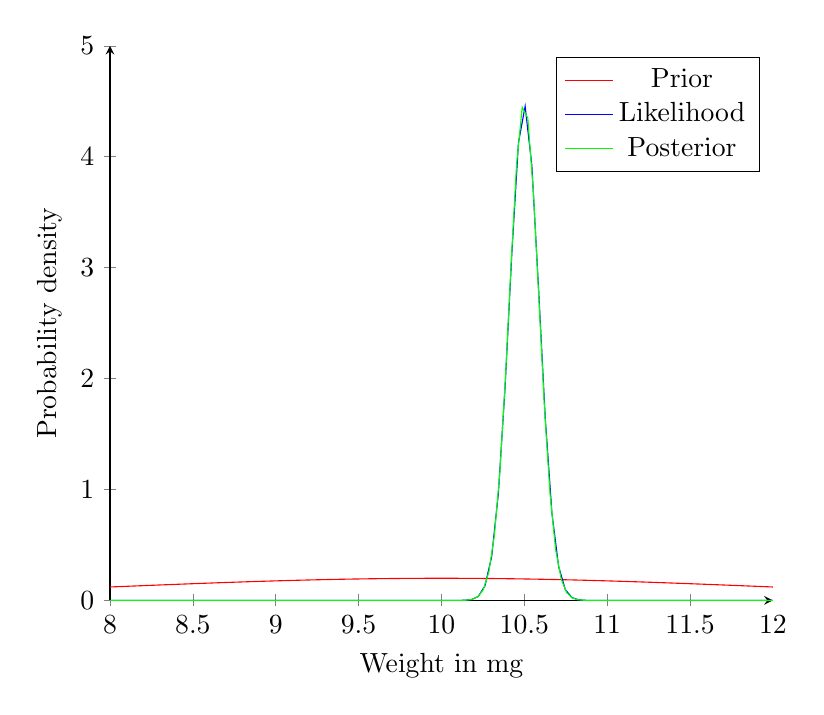
\begin{tikzpicture}
\begin{axis}[
    axis lines = left,
    xlabel = Weight in mg,
    ylabel = Probability density,
    ymin = 0,
    ymax = 5,
]
\addplot [
    domain=8:12, 
    samples=100, 
    color=red,
	]
	{(pow(2.71828, -(x - 10)^2 / (2 * 2^2)) / (pow(2 * 3.14159, 0.5) * 2)};
\addlegendentry{Prior}
\addplot [
    domain=8:12, 
    samples=100, 
    color=blue,
    ]
	{(pow(2.71828, -(x - 10.5)^2 / (2 * 0.08944^2)) / (pow(2 * 3.14159, 0.5) * 0.08944)};
\addlegendentry{Likelihood}
\addplot [
    domain=8:12, 
    samples=120, 
    color=green,
    ]
    {(pow(2.71828, -(x - 10.499)^2 / (2 * 0.089^2)) / (pow(2 * 3.14159, 0.5) * 0.089)};
\addlegendentry{Posterior}
 
\end{axis}
\end{tikzpicture}

The likelihood and posterior are almost indistinguishable in the picture.

\subsection{The prior as quasi-sample}
Unlike the beta distribution, there is no normal distribution which contains no information - The prior will always contain some information. We could consider the limit $\tau\rightarrow\infty$, but this does not correspond to any actual normal distribution. It does turn out, that that following definition captures the equivalent number of samples in the prior well:
\begin{equation}
n_0=\frac{\sigma^2}{\tau^2}
\end{equation}
For starters, the limit $\tau\rightarrow\infty$ means that $n_0$ tends to zero. Let's rewrite the posteriors in terms of $n_0$:
\begin{align}
\mu^*=\frac{\sigma^2\nu+n\tau^2\bar{x}}{\sigma^2+n\tau^2}=\frac{n_0\tau^2\nu+n\tau^2\bar{x}}{n_0\tau^2+n\tau^2}&=\frac{n_0\nu+n\bar{x}}{n_0+n}\\
\sigma^*=\frac{\sigma\tau}{\sqrt{\sigma^2+n\tau^2}}=\frac{\sigma\tau}{\sqrt{n_0\tau^2+n\tau^2}}&=\frac{\sigma}{\sqrt{n_0+n}}
\end{align}
In the limit of $n_0\rightarrow 0$, these turn into the likelihood parameters, and we can draw same conclusion as we did for the beta-binomial conjugate families: The information contained in the prior has equivalent weight to $n_0$ observations.

\subsubsection{Example: Steel beam strength}
Consider the example above once more. Here, the number of quasi-samples is:
\begin{equation}
n_0=\frac{\sigma^2}{\tau^2}=\frac{17.3^2}{10^2}\approx 2.99
\end{equation}
Compare to the 12 real samples - the prior accounts for about one fifth of the information. This is reflected in the associated graphs: The prior affects the posterior somewhat, but the likelihood is more influential.

\subsubsection{Example: Weighing ammonium nitrate}
In the ammonium nitrate example, things are different. Here the number of quasi-samples is:
\begin{equation}
n_0=\frac{\sigma^2}{\tau^2}=\frac{0.2^2}{2^2}=0.01
\end{equation}
So, there's next to no information contained in the prior. This is reflected by the fact that the likelihood and prior are almost identical: The prior doesn't have much effect at all.

\section{Credible intervals}
\textit{Credible intervals} are the Bayesian version of the frequentist confidence intervals. Remember that the interpretation of a confidence interval is, that "95\% of \textit{similarly constructed} intervals will contain the true value". In frequentist statistics, the true parameter actually takes on a certain, true value, and therefore this true value is either in or not it a given confidence interval. In Bayesian statistics this is not so - the parameter itself is a random variable, and therefore there's actually a probability distribution associated with it. Credible intervals can be obtained by the same techniques as is usually used for finding confidence intervals.

\subsection{Credible intervals for beta posteriors}
Here (unless one or both of the parameters happen to be less than one) the extreme values will be around 0 and 1. So there's two critical regions, each containing a probability of half the significance level. The critical values can be easily found in R using the \verb|qbeta| function.

\subsubsection{Example: Radio quality revisited}
\textbf{What is the 95\% credible interval for this example?} The posterior beta distribution had $\alpha=5$ and $\beta=6$ as parameters. The credible interval is found as follows:
\begin{verbatim}
> qbeta(c(0.025, 0.975), shape1 = 5, shape2 = 6)
[1] 0.1870860 0.7376219
\end{verbatim}
This is a rather wide interval, which reflects that the values of the parameters are on the low side.

\subsection{Credible intervals for beta posteriors}
Here, the \verb|qgamma| function can be used with \verb|scale| set to $k$ and \verb|shape| set to $\theta$. For the $\alpha-\beta$-parametrization, use \verb|rate| for $\beta$ instead.

\subsubsection{Example: Workplace accidents}
\textbf{What is the 90\% credible interval for this example?} The posterior gamma distribution has $k=9$ and $\theta=1/8$. So the credible interval is:
\begin{verbatim}
> qgamma(c(0.05, 0.95), shape = 9, scale = 1/8)
[1] 0.5869034 1.8043312
\end{verbatim}

\subsubsection{Example: Cavalrists kicked to death by horses}
\textbf{What is the 99\% credible interval for this example?}
The posterior gamma distribution has $k=3209/16$ and $\theta=4/1203$. The credible interval is:
\begin{verbatim}
> qgamma(c(0.005, 0.995), shape = 3209/16, scale = 4/1203)
[1] 0.5518294 0.7944037
\end{verbatim}

\subsection{Credible intervals for normal posteriors}
Analagously to the previous cases, \verb|qnorm| can be used to find the credible intervals in this case.

\subsubsection{Example: Steel beam strength}
\textbf{What is the 95\% credible interval for this example?} The posterior mean is 68.00 and the posterior standard deviation 4.47. The credible interval is:
\begin{verbatim}
> qnorm(c(0.025, 0.975), mean = 68.00, sd = 4.47)
[1] 59.23896 76.76104
\end{verbatim}

\subsubsection{Example: Weighing ammonium nitrate}
\textbf{What is the 99\% credible interval for this example?} With a posterior mean of 10.499 mg and a posterior standard deviation of 0.089 mg, the credible interval becomes:
\begin{verbatim}
> qnorm(c(0.005, 0.995), mean = 10.499, sd = 0.089)
[1] 10.26975 10.72825
\end{verbatim}

\end{document}
